\emph{This page is for people who want to help develop/improve this
handbook.}

\emph{If you want to get involved, write to
\href{http://en.wikipedia.org/wiki/Howard\_Rheingold}{Howard Rheingold}
at \href{mailto:howard@rheingold.com}{howard@rheingold.com}.}

\emph{Illustrations by \href{http://www.visualsforchange.com/}{Amanda
Lyons}.}

\begin{center}
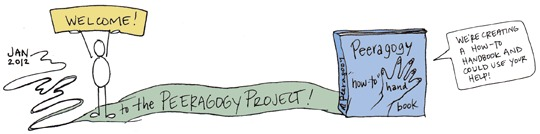
\includegraphics[width=.9\textwidth]{../pictures/welcome_color.jpg}
\end{center}

\subsection{Hello and welcome!}

The peeragogy project was kicked off around the time of
\href{http://rheingold.com/}{Howard Rheingold's} January 23, 2012
\href{http://vimeo.com/35685124}{Regents Lecture} at UC Berkeley on
\emph{Social Media and Peer Learning: From Mediated Pedagogy to
Peeragogy}. We have put together a handbook about peer learning: you're
reading it -- maybe on \href{peeragogy.org}{our website}, or in your
hammock with the beverage of your choice and our
\href{http://www.lulu.com/shop/howard-rheingold-and-peeragogyorg-editors/the-peeragogy-handbook/paperback/product-20607425.html}{print
on demand} paperback. Or maybe you grabbed our
\href{peeragogy-2.0-ebook.pdf}{free PDF} or
some other remixed version in some other format or flavor from some
other place (which would be
\href{http://peeragogy.org/resources/license/}{cool}!).

But: there's still
\href{http://peeragogy.org/peeragogy-org-roadmap/}{more work to be
done}. We created this page because you might be interested in getting
involved in improving the book or furthering the project in other ways.
If so, we're happy to have you aboard!

What you do here is largely up to you. Asking questions is actually
extremely helpful: there's almost always someone in our
\href{https://plus.google.com/u/0/communities/107386162349686249470}{Google+
community} who would be happy to try to answer them, or refer you to
someone else who can.  Or just poke around the public pages on peeragogy.org and
leave a comment or two. Better still, find an area where you feel
knowledgeable -- or are willing to learn -- and start writing (or
filming, dancing, drawing, building, etc.).

\begin{center}
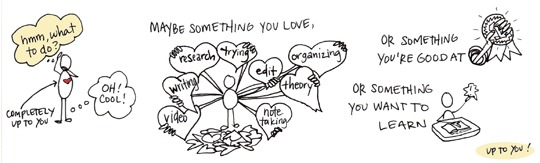
\includegraphics[width=.9\textwidth]{../pictures/what_to_do_color.jpg}
\end{center}

The goal we have in mind for our book is for it be a useful guide to
peer learning! To achieve that goal we have in mind multiple
opportunities for peers to contribute:

\begin{itemize}
\item
  Once we get to know you a little bit we'll be happy to give you a
  login on peeragogy.org and you can start editing and improving this.
\item
  You can go right ahead and post some links to relevant resources,
  either in comments here, or in the G+ or SMC.
\item
  Write the text for a new sub-section (this page was once ``new'' --
  but it's been revised many times by now!).
\item
  We're particularly interested in case studies about
  \href{http://peeragogy.org/peeragogy-in-action/}{Peeragogy in Action}!
\item
  Organize a team to tackle a larger section or topic.
\item
  Make a video (like these on our
  \href{http://www.youtube.com/channel/UCIQY4ja8e4Br-i9U5KnmyZQ}{YouTube
  Channel}),
\item
  Take notes of live meetings, or
  \href{http://cmapspublic3.ihmc.us/rid=1K81VLSK7-1RL0RQ4-WZK/Peeragogy\%20Cmap.cmap}{grow
  concept maps,}
\item
  Organize a newsletter for your group or the whole team,
\item
  Add general purpose bookmarks to
  \href{http://groups.diigo.com/group/peeragogy-handbook}{this Diigo
  group}, or post comments and editorial notes about peeragogy.org in
  \href{http://groups.diigo.com/group/peering-into-peeragogy\%20}{this
  one}; and
\item
  Discuss peer learning matters and this handbook informally with us and
  with others!
\end{itemize}
It's up to you. Instead of worrying too much about
\href{http://peeragogy.org/co-working/}{the rules}, join our
conversations, take advantage of the digital memory of the forum to
rewind the conversation all the way to the beginning (if you want to go
that far), listen in for a little bit if you want to, and jump in
whenever you're ready. We won't know what you're up to until you speak
up. You can have a look at the outstanding tasks and teams that are
listed on
\href{https://docs.google.com/document/d/1\_2I-z-Pt5NUKk-fpy4jsqxFeXbWS4ao4sIhkxCcRVeI/edit\#}{this
Google Doc}: our
\href{http://peeragogy.org/peeragogy-org-roadmap/}{roadmap} is a useful
shared resource too. You can add to these at any time.

We regularly use Google+, Google Hangouts, forums, and email to
communicate asynchronously and pretty much continuously. We also meet
irregularly as a group for synchronous audio-video sessions. Further
details about all these methods of communication can be found below.

In short: here's how it works:


\begin{center}

\includegraphics{../pictures/questions.jpg} \\
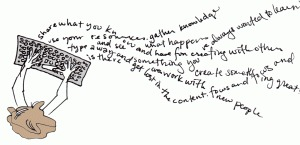
\includegraphics{../pictures/create_content.jpg} \\
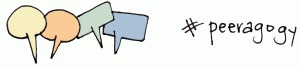
\includegraphics{../pictures/communicate.jpg} \\
\end{center}

\subsection{Questions?}

If you have questions, that's good! Use Google+ or the forums, post a
comment on peeragogy.org, email the team energy center if you know who that
is, or email \href{mailto:howard@rheingold.com}{howard@rheingold.com}.
